% vim:ft=tex

\section{Database}

Since we want to compute distances between the centroids of two postalcode areas we need a database where those information can be stored. 
\subsection{SQL vs NOSql}
First, it was necessary to find a suitable database. For this purpose we compared the \ac{nsql} and the \ac{sql} approaches with each other.\\
\acs{sql} happens to be the more structured, right way of storing data, like a phone book. For a relational database to be effective, you will have to store your data in a
very organized fashion. SQL databases remain popular because they fit naturally into many
vulnerable software stacks, including LAMP and Ruby-based stacks. These databases are widely
supported and well understood, which could be a major plus point if you run into problems.\\
The main problem with SQL is scaling it as your database grows. You see, even though
scalability is usually tested in production environments, it’s often lower than NoSQL
databases.\\\\
For dealing with massive amounts of unstructured data and data requirements which
aren’t clear at the outset, you probably don’t have the luxury of developing a relational database with
a clearly defined schema. You get much more flexibility than its traditional counterparts, with non-
relational databases. Picture non-relational databases as file folders, assembling related information
of all types.\\\\
Since we already know the scope of our database and therefore don`t want to scale it up and due to the lack of time and the good knowledge of team members in SQL, we decided to make use of the relational database \textbf{MySQL}.
\subsection{Installation}
Since MySQL is the most popular open-source relational database management system, we decided to install this system on our server. 
First we installed the MySQL package with the following command:
\begin{lstlisting}[language=bash,breaklines=true]
sudo apt install mysql-server
\end{lstlisting}
Once the installation is completed, the MySQL service will start automatically. To check whether the MySQL server is running or not, we type:
\begin{lstlisting}[language=bash,breaklines=true]
sudo systemctl status mysql
\end{lstlisting}
After we have made sure that the database is running, we create a user account:
\begin{lstlisting}[language=bash,breaklines=true]
CREATE USER IF NOT EXISTS 'database_user'@'localhost' IDENTIFIED BY 'user_password';
Copy
\end{lstlisting}
Afterwards a new database could be created and initialized.
\subsection{Datamodel}
To implement an appropriate database which offers fast responses to queries it was indispensable to design a datamodel which fulfills these requirements. The figure \ref{pic:er} shows the output of the datamodelling process.
\begin{figure}[H]
\hspace{1.2cm}
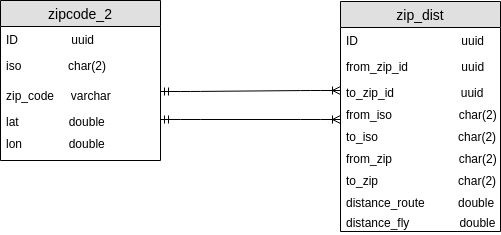
\includegraphics[width=0.8\textwidth]{img/er}
\captionof{figure}{ER model for the MySQL Database}\label{pic:er}
\end{figure}
\noindent The model consists of two entities which are connected over a one-to-many relationship.
The datamodels for the postcodes and the distances were directly written in the Django source code. That way, Django directly provides a python object to work with the tables. It is even possible to write methods to manipulate this data directly from it. The implementation is done in the file:
\href{https://github.com/dataBikeHsUlm/WebApp/blob/master/geonom/datamodel/models.py}{model.py}.
For further information on working with the database in Django, see our corresponding 
\href{https://github.com/dataBikeHsUlm/WebApp/blob/master/django_recap.md#database}{GitHub repository}.
\subsection{Initialize Database}
To be able to fill the postalcode table, we need a list of all postcodes per country. The Nominatim API doesn't directly provide a function to do that, however the \emph{GeoNames}, which is a geographical database, provides a list of all postalcodes which are free to download \citep{GeoNames}.
We implemented a first version of a script using this list and started filling the database.\\
The problem was, some countries (like Greece) were missing and the script had problems finding some cites.  Therefore we had to find another, more reliable way to get the postcodes.
We decided to directly look into the Nominatim PostgreSQL database. There is in fact a table named
\textbf{location\_area} containing the column postcodes and the related \textbf{country\_code} .
Some rows in this table have empty \textbf{country\_code} or \textbf{postcode}, so we need to filter them out. The resulting SQL query looks as followed:
\begin{figure}[H]
\hspace{1.2cm}
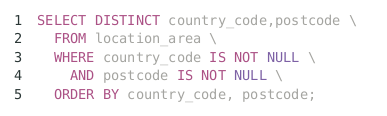
\includegraphics[width=0.55\textwidth]{img/query1}\label{pic:q1}
\end{figure}
\noindent Then, for every postcode, we need to query Nominatim to get the centroid coordinates, but querying only with the country code and the postcode is too ambiguous and can lead to wrong centroids. To fix that, we used the \textbf{country\_name} table that lists countries with names and ISO codes. We joined this table to the previous one:
\begin{figure}[H]
\hspace{1.2cm}
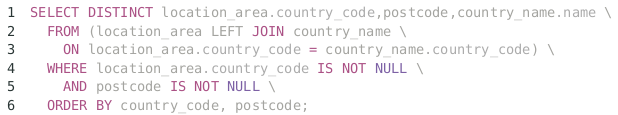
\includegraphics[width=0.9\textwidth]{img/query2}\label{pic:q2}
\end{figure}
\noindent Using the resulting data, the script to fill the zipcode table was re-written, the database cleaned and filled with the new version of the script. The script can be found at the GitHub repository \href{https://github.com/dataBikeHsUlm/WebApp/blob/master/fill_db_from_osm.py}{WebApp}. \\To run the script, run the accompanying shell script \textbf{fill\_db.py}, it will install the dependencies before running the python code.
